\documentclass[12pt,a4paper,oneside]{report}             % Single-side
%\documentclass[12pt,a4paper,twoside,openright]{report}  % Duplex

%\PassOptionsToPackage{chapternumber=Huordinal}{magyar.ldf}
\usepackage{bm}
\usepackage{amsmath}
\usepackage{amssymb}
\usepackage{enumerate}
\usepackage[thmmarks]{ntheorem}
\usepackage{graphics}
\usepackage{epsfig}
\usepackage{listings}
\usepackage{color}
\usepackage{algorithm}
\usepackage{algorithmic}
\usepackage{lastpage}
\usepackage{anysize}
\usepackage{sectsty}
\usepackage{setspace}  % Ettol a tablazatok, abrak, labjegyzetek maradnak 1-es sorkozzel!
\usepackage[hang]{caption}
\usepackage{hyperref}
\usepackage[magyar]{babel}
\usepackage{fontspec}
\usepackage{textcomp}
\usepackage{subcaption}
\usepackage{titlesec, blindtext, color}
\usepackage{fancyhdr}
\usepackage{lastpage}
\usepackage{todonotes}
\usepackage{graphicx}
\usepackage{tikz}
\usepackage{subcaption}
\usepackage{float}
\usepackage{listings}
\usepackage{xcolor}
\usepackage[sorting=none, backend=biber, style=ieee]{biblatex}
\usepackage{courier}
\addbibresource{bib.bib}
\lstloadaspects{formats}

\definecolor{commentgreen}{RGB}{0,200,10}
\definecolor{weborange}{RGB}{255,10,0}
\definecolor{frenchplum}{RGB}{129,20,83}
\definecolor{codegray}{rgb}{0.5,0.5,0.5}
\definecolor{backcolour}{rgb}{0.95,0.95,0.92}

\setlength{\headheight}{14.5pt}

\lstdefinestyle{mystyle}{
	backgroundcolor=\color{backcolour},   
	commentstyle=\color{codegray},
	keywordstyle=\bf\color{frenchplum},
	numberstyle=\color{frenchplum},
	stringstyle=\color{commentgreen},
	basicstyle=\ttfamily\footnotesize,
	breakatwhitespace=false, 
	fontadjust=true,        
	breaklines=true,                 
	captionpos=b,
	columns=flexible,                   
	keepspaces=true,                 
	numbers=none,                    
	numbersep=5pt,                  
	showspaces=false,                
	showstringspaces=false,
	showtabs=false,                 
	tabsize=4
}

\lstset{style=mystyle}

%--------------------------------------------------------------------------------------
% Main variables
%--------------------------------------------------------------------------------------
\newcommand{\vikauthor}{Szemenyei Márton}
\newcommand{\viktitle}{M9 – Szegmentálás mély neurális hálókkal}
\newcommand{\vikdept}{Irányítástechnika és Informatika Tanszék}
\newcommand{\vikdoktipus}{Irányítástechnika és Képfeldolgozás Laboratórium 1.}
\newcommand{\viksubtitle}{Mérési Útmutató}

%--------------------------------------------------------------------------------------
% Page layout setup
%--------------------------------------------------------------------------------------
% we need to redefine the pagestyle plain
% another possibility is to use the body of this command without \fancypagestyle
% and use \pagestyle{fancy} but in that case the special pages
% (like the ToC, the References, and the Chapter pages)remain in plane style

\pagestyle{plain}
\setlength{\parindent}{0pt} % �ttekinthet�bb, angol nyelv� dokumentumokban jellemz�
\setlength{\parskip}{8pt plus 3pt minus 3pt} % �ttekinthet�bb, angol nyelv� dokumentumokban jellemz�
%\setlength{\parindent}{12pt} % magyar nyelv� dokumentumokban jellemz�
%\setlength{\parskip}{0pt}    % magyar nyelv� dokumentumokban jellemz�

\marginsize{35mm}{25mm}{15mm}{15mm} % anysize package
\setcounter{secnumdepth}{0}
\sectionfont{\large\upshape\bfseries}
\setcounter{secnumdepth}{2}

%--------------------------------------------------------------------------------------
%	Setup hyperref package
%--------------------------------------------------------------------------------------
\hypersetup{
    pdftitle={\viktitle},        % title
    pdfauthor={\vikauthor},    % author
    pdfsubject={\vikdoktipus}, % subject of the document
    pdfcreator={\vikauthor},   % creator of the document
    pdfkeywords={Számítógépes látás, Neurális Háló. Deep Learning, Osztályozás},    % list of keywords
    pdfnewwindow=true,         % links in new window
    colorlinks=true,           % false: boxed links; true: colored links
    linkcolor=black,           % color of internal links
    citecolor=black,           % color of links to bibliography
    filecolor=black,           % color of file links
    urlcolor=black             % color of external links
}	

%--------------------------------------------------------------------------------------
%	Some new commands and declarations
%--------------------------------------------------------------------------------------
\newcommand{\code}[1]{{\upshape\ttfamily\scriptsize\indent #1}}

% define references
\newcommand{\figref}[1]{\ref{fig:#1}.}
\renewcommand{\eqref}[1]{(\ref{eq:#1})}
\newcommand{\listref}[1]{\ref{listing:#1}.}
\newcommand{\sectref}[1]{\ref{sect:#1}}
\newcommand{\tabref}[1]{\ref{tab:#1}.}

\DeclareMathOperator*{\argmax}{arg\,max}
%\DeclareMathOperator*[1]{\floor}{arg\,max}
\DeclareMathOperator{\sign}{sgn}
\DeclareMathOperator{\rot}{rot}
\definecolor{lightgray}{rgb}{0.95,0.95,0.95}

\newcommand{\hsp}{\hspace{20pt}}
\titleformat{\chapter}[hang]{\Huge\bfseries}{\thechapter\hsp}{0pt}{\Huge\bfseries}
\titlespacing*{\chapter}{0pt}{0pt}{40pt}


\author{\vikauthor}
\title{\viktitle}
%--------------------------------------------------------------------------------------
%	Setup captions
%--------------------------------------------------------------------------------------
\captionsetup[figure]{
%labelsep=none,
%font={footnotesize,it},
%justification=justified,
width=.9\textwidth,
aboveskip=10pt}

\renewcommand{\captionlabelfont}{\small\bf}
\renewcommand{\captionfont}{\footnotesize\it}

\fancypagestyle{plain}{%
	\fancyhf{}
	\renewcommand{\footrulewidth}{1pt}
	\chead{\viktitle}
	\lfoot{\thepage/\pageref{LastPage}} %/\pagetotal
	\rfoot{\leftmark}
}
\pagestyle{plain}

\pagestyle{fancy}
\renewcommand{\chaptermark}[1]{\markboth{\MakeUppercase{#1}}{}}
\fancyhf{}
\chead{\viktitle}
\lfoot{\thepage/\pageref{LastPage}} %/\pagetotal
\rfoot{\leftmark}
\renewcommand{\footrulewidth}{1pt}

%--------------------------------------------------------------------------------------
% Table of contents and the main text
%--------------------------------------------------------------------------------------
\begin{document}

\onehalfspacing

%--------------------------------------------------------------------------------------
%	The title page
%--------------------------------------------------------------------------------------
\begin{titlepage}
\begin{center}

\includegraphics[width=60mm,keepaspectratio]{images/logo.png}\\
\vspace{0.3cm}
\textbf{Budapesti Műszaki és Gazdaságtudományi Egyetem}\\
\textmd{Villamosmérnöki és Informatikai Kar}\\
\textmd{\vikdept}\\[5cm]

\vspace{0.4cm}
{\huge \bfseries \viktitle}\\[2cm]
\textsc{\Large \viksubtitle}\\[1cm]
\textsc{\Large \vikdoktipus}\\[6cm]

\vfill
{\large \vikauthor}
\end{center}
\end{titlepage}

%\pagenumbering{arabic}

%--------------------------------------------------------------------------------------
% tartalom, ábra és táblázatjegyzék
%--------------------------------------------------------------------------------------
\singlespacing
\tableofcontents\thispagestyle{fancy}
\titleformat{\chapter}[hang]{\Huge\bfseries}{\thechapter\hsp}{0pt}{\Huge\bfseries}
\onehalfspacing

\chapter{Neurális hálók}

A számítógépes látás a számítástudomány egyik legrohamosabban fejlődő területe, amelynek egyre több gyakorlati felhasználása létezik. Ez a tendencia nem meglepő, hiszen az ember az érzékszervei közül a szemre hagyatkozik a leginkább a napi feladatinak ellátásakor. Ebből következik, hogy ha a számítógépes látás algoritmusai képesek megközelíteni, vagy akár felülmúlni az emberi látás képességeit, akkor számos fontos feladatot leszünk képesek automatizálni. Könnyen belátható azonban az is, hogy a gyakorlatban ez egy rendkívül nehéz feladat, mivel általában olyan feladatokat tudunk könnyedén algoritmusok formájában leírni, ahol a feladat elvégzésének a menetét pontosan, tudatos szinten megértjük. A szemből érkező jelek feldolgozásának azonban a jelentős része tudatalatti szinten történik, így aligha tudjuk ezeket a folyamatokat könnyedén megérteni, és algoritmusok formájában lemásolni.

Ennek a problémának a megoldásához a mesterséges intelligencia, ezen belül is a gépi tanulás módszereihez kell nyúlnunk. A tanuló számítógépes látás legegyszerűbb formája az osztályozás, vagyis amikor egy képhez egyetlen címkét rendelünk, amely a képen található objektum kategóriáját kódolja. Bizonyos esetekben a címke mellé már egy az adott objektumot körbefogó téglalapot is rendelünk, ebben az esetben lokalizációról beszélhetünk. Adott esetben ennél magasabb szintű információt is szeretnénk kinyerni a képből: érdekelhet minket az, hogy melyek azok a pixelek az adott képen, amelyek az észlelt osztályhoz tartoznak. Amennyiben ezt az információt egy képsorozaton minden pixelre meghatározzuk, akkor követésről beszélhetünk.

A neurális hálózatokról és azok tanításáról bővebben a Számítógépes Látórendszerek c. tárgy jegyzetében~\cite{szgl} olvashatunk.

\section{Az EfficientNet architektúra}

Az EfficientNet~\cite{effnet} egy olyan konvolúciós neurális háló architektúra, amelyet automatikus optimalizáló eljárással (ún. Neural Architecture Search~\cite{nas} módszerrel) fejlesztettek ki. Ez egy olyan eljáráa, ahol egy megerősítéses tanulás ágenst arra tanítanak, hogy minél jobb neurális háló architektúrákat generáljon. Itt a jóság alatt a háló elért pontossága és az architektúra gyorsasága közötti valamilyen kompromisszumot értjük. Ezt jól illusztrálja az alábbi ábra:

\begin{figure}[H]
	\centering
	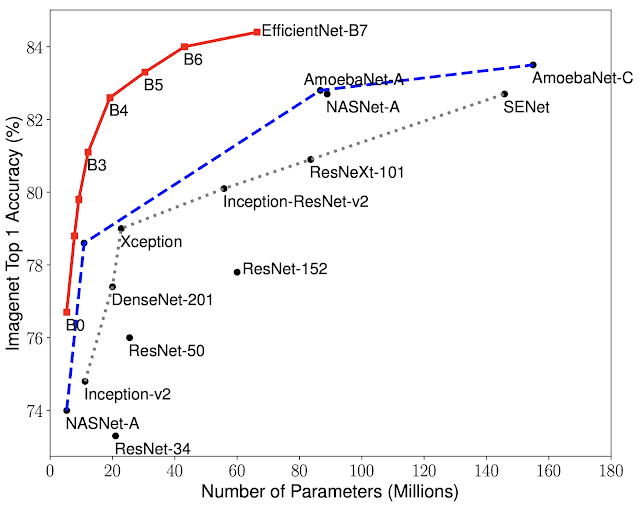
\includegraphics[width=0.9\textwidth]{images/effnet.png}
	\caption{Az EfficientNet architektúra pontossága az ImageNet adatbázison a paraméterszám függvényében, más hálózatokkal összehasonlítva.}
\end{figure}

Az EfficientNet architektúra implementálása maga nem a mérés része, azonban a konvolúciós blokkot érdemes vizsgálni, ugyanis ebben a korábban megismert trükkök közül több is megtalálható. Az EfficientNet alapvető blokkja ugyanis egy bottleneck-et tartalmazó reziduális blokk, amelynek fő konvolúciós eleme (amelyik $5\times 5$ kiterjedésű) aszimmetrikus. Ez azt jelenti, hogy egy darab $5\times 5$ konvolúció helyett egy $5\times 1$ és egy $1\times 5$ konvolúciót hajtunk végre egymás után. Ennek számítási igénye $O(5\times 5\times ch)$ helyett $O(2\times 5\times ch)$.

\chapter{A mérés környezete}

A mérés során a \emph{PyCharm} elnevezésű IDE áll rendelkezésre, amely rendkívül sokoldalú szolgáltatásokkal könnyíti meg a szoftverfejlesztést, például konfigurálható automatikus formázási lehetőségek állnak rendelkezésünkre. További részletekért érdemes lehet a JetBrains ide vonatkozó weboldalát~\cite{pycharm} felkeresni. Függvények, objektumok esetében a \textbf{\textit{Ctrl+P}} billentyűkombináció pop-up segítségként szolgálva mutatja nekünk a paramétereket. A mérés során használt programnyelv a Python 3-as verziója lesz.

A Python programnyelvhez számos hasznos függvénykönyvtár tartozik, melyek a mérési feladatok megvalósítását nagymértékben megkönnyítik. A Python nyelv egyik rendkívül kényelmes funkciója a beépített package manager, amelynek segítségével az egyes könyvtárak automatikusan telepíthetők, telepítsük után pedig minden további beállítás nélkül használhatók. A Pythonhoz két ilyen package manager is tartozik, az egyik a Pip, amely a legtöbb telepíthető Python verzió mellé automatikusan települ, a másik pedig az Anaconda~\cite{conda}, ami a könyvtárkezelési funkciókon túl virtuális környezeteket is képes kezelni.

A Python egyik legfontosabb függvénykönyvtára a Numpy, amely tömbök kezelésére, illetve számtalan numerikus algoritmus használatára ad lehetőséget. A Numpy funkcionalitását kiegészíti a MatplotLib, melynek segítségével különböző ábrákat készíthetünk a tömbjeinkről. Egy harmadik rendkívül hasznos könyvtárcsalád a scikit, ami számos tudományos számításhoz szükséges alkönyvtárt foglal össze. A sckit-image képek kezelésére, a scikit-learn gépi tanulás algoritmusok használatára, míg a scikit-fuzzy fuzzy logika használatára ad lehetőséget. Ezek a könyvtárak tulajdonképpen együttesen kiadják a Matlab funkcionalitásának jelentős részét.

\section{PyTorch}

A PyTorch~\cite{torchDoc,torchTut} a Facebook Research által fejlesztett Deep Learning keretrendszer, melyet a mérés során használni fogunk, így a következőkben röviden áttekintésre kerülnek a fontosabb koncepciók. A PyTorch egyik előnye a TensorFlow-val, Keras-szal szemben, hogy a hálózatot leíró gráf dinamikusan kerül létrehozásra, nincs fordítási szakasza a tanításnak – ez a kevesebb lépés mellett akár azt is lehetővé teszi számunkra, hogy a háló rétegeit tanítás közben változtassuk (mert az egyik hiperparaméterünk lehet a lineáris rétegek száma).

A PyTorch alapja az akár GPU-n is futtatható tenzor típus, mely egy pratikus tagfüggvényekkel felvértezett, multidimenzionális tömböt megvalósító osztály – tehát felettébb alkalmas például képek tárolására is.

Tenzorokon alapul a rétegeket/hálózatokat megvalósító Module osztály, melyből minden saját hálózatunknak örökölnie kell, így kerülnek regisztrálásra az előre-, ill. visszaterjesztést megvalósító függvényeink. Szerencsére nem kell a hibavisszaterjesztést kézzel megírni, a PyTorvh beépített automatikus differenciálásra képes modulja (autograd) megteszi ezt helyettünk.

Fontos megjegyezni, hogy az automatikus differenciálás nem szimbolikus differenciálás (azaz nem az a célja, hogy paraméteresen felírja egy bonyolult összefüggés deriváltfüggvényét) és nem is numerikus differenciálás (tehát az sem cél, hogy iteratívan közelítsünk egy értéket, mert a kvantálás/kerekítés jelentős eltérésekben nyilvánulhat meg). Automatikus differenciálás során egy számítási gráf segítségével, a láncszabályt alkalmazva vagyunk képesek, viszonylag jól skálázhatóan, parciális deriváltakat kiszámítani, ami feltétlenül szükséges gradiens-alapú tanulóalgoritmusok esetében.

A PyTorch optim nevű almodulja tartalmazza a különböző, a tanítás során használt algoritmusokat, ezek közül nekünk most csak az SGD-re (stochastic gradient descent) lesz szükségünk. Az SGD objektum számára megadható a modell, a tanulási ráta (learning rate), a momentum, ill. van lehetőség normán alapuló regularizáció konfigurálására is.

Ahhoz, hogy tanítani tudjunk egy hálózatot, a következő struktúrájú programot kell megvalósítanunk és iteratívan meghívnunk. A következőkben a PyTorch egyik kiegészítésének (Ignite) forráskódjából látható egy részlet, ami tömören magába foglalja a szükséges lépéseket – a mérésen ugyanezen lépések segítségével, de egy kicsit más struktúrában fogjuk a tanítást végezni.

\begin{lstlisting}[language=Python]
def _update(batch):
	model.train()
	optimizer.zero_grad()
	x, y = _prepare_batch(batch, device=device)
	y_pred = model(x)
	loss = loss_fn(y_pred, y)
	loss.backward()
	optimizer.step()
	return loss.item()
\end{lstlisting}

Részleteiben a következő történik: tudatnunk kell a programmal, hogy most tanítjuk a hálót (hogy pl. a dropout csak ilyen esetben kerüljön aktiválásra). Ezt követően a gradiensek előző értékét kell nulláznunk (ugyanis megtehetnénk, hogy valamihez még felhasználjuk, ezért nem történik automatikusan). Ahhoz, hogy a következő előreterjesztést véghez vihessük, elő kell készíteni a következő minibatchet (ezt a kódban egy saját függvény, \_prepare\_batch jelöli). Az előreterjesztés végrehajtása felettébb egyszerű, magának a modellnek adjuk át argumentumként a minibatchet. A hiba kiszámítása a következő lépés, ezt az általunk konfigurált hibafüggvény segítségével tehetjük meg, majd a hiba backward tagfüggvényét meghívva végrehajtjuk a hibavisszaterjesztést. Nagyon fontos az utolsó lépés az optimalizáló algoritmus (SGD) lépésének végrehajtása, így kerülnek a súlyok frissítésre.

Számos gyakran használt adatbázis elérhető a torchvision modulból, ezek előkészítésére, ill. adat augmentációra is használható transzformációk is rendelkezésünkre állnak. Ezen felül van lehetőség DataLoader objektumok segítségével (torch.utils.data modul) az adatok betöltését automatizálni. Továbbá lehetőségünk van például a tanulási ráta automatikus megváltoztatására adott szabályrendszer szerint.

\section{Haladó Python}

A korábbi mérés(ek) során megismerkedtünk a Python nyelvvel, a jelen mérés során azonban a nyelv bonyolultabb funkcióira is szükségünk lesz. Az alábbiakban tekintsük át legfontosabb adattípusokat és nyelvi elemeket.

A Python legfontosabb konténer osztályai a list és a tuple. Ezek közt a különbség, hogy a tuple immutable, vagyis nem módosítható. Létrehozásuk és az elemeik elérése az alábbi módon történhet:

\begin{lstlisting}[language=Python]
myList = ["wow","you","can","mix",2,"or","more","different","types"]
myTuple = ("wow","you","can","mix",2,"or","more","different","types")
myList[4] = "two" # 2 becomes 'two'
myTuple[4] = "two" # Error
\end{lstlisting}

Érdemes tudni, hogy habár (1D) listák esetében a $+$ operátor értelmezett, ez a listákat összefűzi, nem pedig összeadja.

\begin{lstlisting}[language=Python]
myList = [1,2]+[3,4]
>>> [1,2,3,4] # Not [4,5]
\end{lstlisting}

Listákhoz új elemet az alábbi módon lehet hozzáadni:

\begin{lstlisting}[language=Python]
myList = [1,2,3,4]
myList.append(5) # [1,2,3,4,5]
\end{lstlisting}

Listák, vagy Tuple-ök elemein az alábbi módokon lehet végigiterálni:

\begin{lstlisting}[language=Python]
for elem in myList:
print(elem)

for i, elem in enumerate(myList):
print(i,elem) # i is the index
\end{lstlisting}

Adott esetben egyszerre több (egyenlő elemszámú) listán is végigiterálhatunk egyidejűleg:

\begin{lstlisting}[language=Python]
if len(list1) == len(list2):
for (elem1,elem2) in zip(list1,list2):
print(elem1,elem2)
\end{lstlisting}

Érdemes megjegyezni, hogy az 'in' kulcsszó feltételeknél is használható annak eldöntésére, hogy egy adott érték szerepel-e a listában:

\begin{lstlisting}[language=Python]
myList = [1,2,3,4]
if 1 in myList:
print("1 is in the list")
if 5 not in myList:
print("5 is not in the list")
\end{lstlisting}

A Python programnyelv támogat bizonyos funkcionális programozási elemeket is, melyek közül az egyik leghasznosabb az úgynevezett list comprehension. Ezt akkor használhatjuk, ha szeretnénk egy lista minden elemén elvégezni egy műveletet és ezek eredményeiből egy újabb listát készíteni. Az alábbi példa egy lista minden elemét négyzetre emeli:

\begin{lstlisting}[language=Python]
myList = [1,2,3,4]
mySqrList = [elem**2 for elem in myList] # [1,4,9,16]
\end{lstlisting}

A list comprehension a korábban említett for ciklus változatokkal (zip, enumerate) is használható, az új lista elemének kiszámolásához pedig bármilyen érvényes Python kód írható. Ezen felül a kifejezés feltétellel is kiegészíthető:

\begin{lstlisting}[language=Python]
myList = [9,-16,25,-4]
mySqrtList = [sqrt(elem) for elem in myList if elem >= 0] # [3,5]
\end{lstlisting}

\section{Haladó NumPy}

Fontos megjegyezni, hogy a Python list és tuple osztályok különböző típusú objektumokat tartalmazhatnak, vagyis egy lista egyik eleme lehet egy másik lista. Ez lehetőséget nyújt arra, hogy a lista osztályt N-dimenziós tömbként használjuk, azonban egy listákat tartalmazó listában az egyes részlisták különböző hosszúak és típusúak lehetnek, ami hagyományos tömböknél nem fordulhat elő. Éppen ezért méret- és típus konzisztens tömbök tárolására a NumPy array osztályt célszerű használni.

A NumPy tömbök között definiált a $+$, $-$, $*$ és a $/$ művelete, azonban ezeket elemenként végzi, így a tömbök méretének kompatibilisnek kell lennie. A NumPy broadcasting szabályai alapján két tömb az alábbi feltételek teljesítése esetén kompatibilis méretű:

\begin{enumerate}
	\item A két tömb minden mérete megegyezik
	\item Amelyik dimenzió mentén nem egyeznek meg a méretek, ott az egyik tömb mérete 1
\end{enumerate}

A tömbök méretét az alábbi módon ellenőrizhetjük:

\begin{lstlisting}[language=Python]
arr1.shape # [2,4,6]
arr2.shape # [1,4,1] - Compatible
arr3.shape # [3,4,6] - Incompatible
\end{lstlisting}

Bizonyos esetekben előfordulhat, hogy új elemet szeretnénk a tömbhöz adni, vagy két tömböt össze szeretnénk fűzni, amelyeket az alábbi módon tehetünk meg:

\begin{lstlisting}[language=Python]
extArr = np.append(arr,elem,dim)
catArr = np.concatenate((arr1,arr2,...,arrn),dim)
\end{lstlisting}

A $dim$ változó azt adja meg, hogy melyik dimenzió mentén történjen a kiegészítés/összefűzés. Ha None értéket adunk meg (nem adjuk meg a paramétert), akkor a NumPy megpróbálja magától kitalálni.

Gyakran előfordul, hogy egy általunk használt tömbben van egy extra dimenzió, aminek az értéke egy. Például, ha van egy 2D mátrixokból álló tömbünk, amelyiknek kivesszük egy elemét. Ez az extra dimenzió sok fejfájást tud okozni, mert ha konkatenálni, vagy mátrixokat szorozni szeretnénk, a NumPy nem megfelelő méret hibákat fog dobni. Ennek megoldására a squeeze parancs való.

\begin{lstlisting}[language=Python]
mtxArr.shape # [N,3,3] - N 3x3 matrices
myMtx = mtxArr[i]
myMtx.shape # [1,3,3]
myMtx = mtxArr[i].squeeze()
myMtx.shape # [3,3]
\end{lstlisting}

Előfordulhat az is, hogy a tömbjeink megfelelő méretűek, de valamilyen oknál fogva a dimenziók sorrendje eltér. Például képek esetén elterjedt konvenció a $H\times W\times Ch$ sorrend használata, a Deep Learning könyvtárak viszont a $Ch\times H\times W$ sorrendet preferálják. Erre megoldás a NumPy transpose függvény.

\begin{lstlisting}[language=Python]
myArr.shape # [N,3]
np.transpose(myArr).shape # [3,N]

# Több dimenzióban
myImg.shape # [1080,1920,3]
np.transpose(myImg,(2,0,1)).shape # [3,1080,1920]
\end{lstlisting}

Ezen felül érdemes még említeni, hogy a NumPy képes különböző lineáris algebrai műveletek elvégzésére, mint például a mátrixszorzás (amennyiben a dimenziók megfelelőek), valamint az invertálás:

\begin{lstlisting}[language=Python]
myMtx = np.array([[1,2,3],[4,5,6],[7,8,9]])
myInv = np.linalg.inv(myMtx)

myData = np.randn((50,3)) # 50 3D coordinates
myTrData = np.matMul(myMtx,myData) # myTrData = myMtx*myData
\end{lstlisting}

Fontos megemlíteni, hogy a $numpy.ndarray$ típuson elvégezhető műveletek nagy része pontosan ugyanúgy működik $torch.tensor$ típuson is, bár esetenként ugyanaz a függvény más néven érhető el. A $numpy.transpose$ például $torch.permute$.

\chapter{Mérési feladatok}

A mérés folyamán az alábbi feladatokat kell elvégezni:

\begin{enumerate}
\item Egészítse ki a mellékelt notebookban megadott adatbázis beolvasót adataugmentációs eljárásokkal.
\item Implementálja le az EfficientNet architektúra alapvető konvolúciós blokkját, és az asszimetrikus reziduális blokkját.
\item Készítsen eljárást egyszerű neurális háló tanítására a méréshez használt adatbázison.
\item Végezzen el különböző tanításokat a \ref{tab:2}.~Táblázatban megadott hiperparaméterek alapján, értékelje ezek eredményeit.
\end{enumerate}

\begin{table}[!htb]
\centering
\begin{tabular}{| c | c | c | c | c | c |}
	\hline
	epochs & lr\_decay\_epochs & batch\_size & lr & lr\_decay & weight\_decay \\ \hline \hline
	20 & 10 & 8 & 5e-4 & 0.1 &  2e-4  \\ \hline
	20 & 10 & 8 & 1e-1 & 0.1 & 2e-4 \\ \hline
	20 & 10 & 8 & 5e-4 & 0.001 &  2e-4  \\ \hline
	20 & 10 & 8 & 5e-4 & 0.1 &  1e-1  \\ \hline
	20 & 10 & 2 & 5e-4 & 0.1 &  2e-4   \\ \hline
	100 & 50 & 8 & 5e-4 & 0.1 &  2e-4  \\ \hline
\end{tabular}
\caption{A Vizsgálandó hiperparaméter kombinációk.}
\label{tab:2}
\end{table}

\chapter{Hasznos kódrészletek}

Érték elérése az argumentumokból

\begin{lstlisting}[language=Python]
myVal = args["arg_name"]
\end{lstlisting}

Tenzor tükrözése a vízszintes tengely mentén (utolsó dimenzió)

\begin{lstlisting}[language=Python]
tensor = tensor.flip(-1)
\end{lstlisting}

Transzformációk kompozíciója

\begin{lstlisting}[language=Python]
image_transform = transforms.Compose(
	[transform1,
	transform2]
)
\end{lstlisting}

Átméretezés transzformáció

\begin{lstlisting}[language=Python]
transforms.Resize((height, width), INTER_MODE)
#Interpolation can be Image.LINEAR or Image.NEAREST
\end{lstlisting}

Tenzor konverzió

\begin{lstlisting}[language=Python]
# To float tensor (for images)
transforms.ToTensor()
# To long tensor (for labels)
ext_transforms.PILToLongTensor()
\end{lstlisting}

Dataloader létrehozása

\begin{lstlisting}[language=Python]
dataLoader = torch.utils.data.DataLoader(trainSet, batch_size=..., shuffle=True/False, num_workers=...)
\end{lstlisting}

Neurális háló módjainak állítása

\begin{lstlisting}[language=Python]
net.train()
net.eval()
\end{lstlisting}
	
Optimizer kinullázása
	
\begin{lstlisting}[language=Python]
optimizer.zero_grad()
\end{lstlisting}
	
Forward

\begin{lstlisting}[language=Python]
outputs = net(inputs)
\end{lstlisting}

Költség

\begin{lstlisting}[language=Python]
loss = criterion(outputs, labels)
\end{lstlisting}

Backward

\begin{lstlisting}[language=Python]
loss.backward()
\end{lstlisting}

Egy lépés gradiens módszerrel

\begin{lstlisting}[language=Python]
optimizer.step()
\end{lstlisting}

Gradiens számítás megelőzése

\begin{lstlisting}[language=Python]
with torch.no_grad():
\end{lstlisting}

Különböző rétegek létrehozása PyTorch környezeteben

\begin{lstlisting}[language=Python]
self.conv = nn.Conv2d(...)
self.bn = nn.BatchNorm2d(...)
\end{lstlisting}

Rétegek kombinálása

\begin{lstlisting}[language=Python]
self.combined = nn.Sequential(layer_1,layer_2,)
\end{lstlisting}

Rétegek meghívása

\begin{lstlisting}[language=Python]
out = self.layer_name(in)
\end{lstlisting}

Tenzor/Modell átvitele a megfelelő eszközre (GPU/CPU)

\begin{lstlisting}[language=Python]
model = model.to(self.device)
\end{lstlisting}

Költségfüggvény létrehozása

\begin{lstlisting}[language=Python]
criterion = nn.CrossEntropyLoss(weight=...)
\end{lstlisting}

Optimalizáló módszer létrehozás

\begin{lstlisting}[language=Python]
optimizer = optim.Adam(model.parameters(), lr=..., weight_decay=...)
\end{lstlisting}

Tanulási ráta ütemező létrehozása

\begin{lstlisting}[language=Python]
lr_updater = lr_scheduler.StepLR(optimizer, <lr_decay_epochs>, <lr_decay>)
\end{lstlisting}


\chapter{Ellenőrző kérdések}

\begin{enumerate}
\item Ismertesse röviden a Hinge és a Kereszt-entrópia költségfüggvényeket! Mi az előnyük/hátrányuk?
\item Hogyan működik a gradiens módszer? Milyen fontos kiegészítései vannak?
\item Mire való a backpropagation? Hogyan működik?
\item Ismertesse egy konvolúciós háló és gyakori rétegei felépítését!
\item Milyen módszerekkel kerülhető el az overfitting? Ismertesse ezeket egy-egy mondatban!
\item Milyen módszerekkel javítható egy neurális háló konvergenciája? Ismertesse ezeket egy-egy mondatban!
\item Ismertesse röviden a PyTorch könyvtárat! Milyen alapvető adattípusai, moduljai léteznek? Milyen szolgáltatásokat nyújt neurális hálók számára?
\item Készítsen egy egyszerű szkriptet Python nyelven: 
\begin{enumerate}
\item Töltse be a torch könyvtár nn nevű modulját!
\item Definiáljon egy új, MyNet nevű osztályt, melynek ősosztálya az nn.Module
\item Az osztály konstruktorában hozzon létre egy mult nevű tagváltozót, értéke legyen 5.
\item Definiáljon egy forward nevű tagfüggvényt, melynek bemeneti paramétere x, és a mult nevű tagváltozóval szorozza meg, az eredményt pedig adja vissza.
\end{enumerate}
\item Hogyan néz ki egyetlen tanulási ciklus PyTorch-ban? (Pszeudó kód elég)
\end{enumerate}


\printbibliography

\end{document}

